\caulc
\begin{ex}%[1D6N3-2]%[TDMZZ22]%[Phạm Hải Dương]
	Tập xác định của hàm số $y=\log_2(1-x)$ là
	\choice
	{\True $(-\infty;1)$}
	{$\mathbb{R}\setminus\{1\}$}
	{$(0;1)$}
	{$(1;+\infty)$}
	\loigiai{
		Hàm số xác định khi và chỉ khi $1-x>0 \Leftrightarrow x<1$.\\
		Vậy tập xác định của hàm số là $\mathscr{D}=(-\infty;1)$.
	}
\end{ex}

\begin{ex}%[1D6H4-5]%[TDMZZ22]%[Phạm Hải Dương]
	Tập nghiệm của bất phương trình $2^{x^2-x+1}\le 8$ là
	\choice
	{$0<x\le 2$}
	{$x\le -1$}
	{$x\ge 3$}
	{\True $-1\le x\le 2$}
	\loigiai{
		Ta có \[2^{x^2-x+1}\le 8 \Leftrightarrow 2^{x^2-x+1}\le 2^3 \Leftrightarrow x^2-x+1\le 3 \Leftrightarrow x^2-x-2\le 0 \Leftrightarrow -1\le x\le 2.\]
		Vậy tập nghiệm của bất phương trình là $S=[-1;2]$.
	}
\end{ex}

\begin{ex}%[1H8N7-2]%[TDMZZ22]%[Phạm Hải Dương]
	Cho hình chóp $S. ABC$ có đáy $ABC$ là tam giác đều cạnh $a$ và khoảng cách từ đỉnh $S$ xuống đáy $\left(ABC\right)$ bằng $3a$.
	\begin{center}
		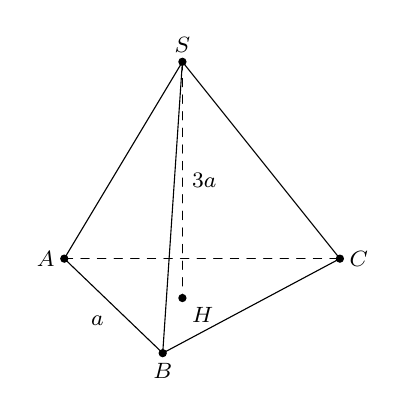
\begin{tikzpicture}[scale=1, font=\footnotesize, line join=round,line cap=round, >=stealth]
			\coordinate (A) at (0,0);
			\coordinate (B) at (1.25,-1.2);
			\coordinate (C) at (3.5,0);
			\coordinate (H) at (1.5,-0.5);
			\coordinate (S) at (1.5,2.5);		
			\draw (S)--(A)--(B)--(C)--(S)--(B);
			\draw[dashed] (A)--(C) (S)--(H);		
			\fill (A) circle (1.5pt) node[left] {$A$};
			\fill (B) circle (1.5pt) node[below] {$B$};
			\fill (C) circle (1.5pt) node[right] {$C$};
			\fill (H) circle (1.5pt) node[below right] {$H$};
			\fill (S) circle (1.5pt) node[above] {$S$};		
			\path (A)--(B) node[midway, below left] {$a$};
			\path (S)--(H) node[midway, right] {$3a$};
		\end{tikzpicture}
	\end{center}
	Thể tích khối chóp $S. ABC$ bằng
	\choice
	{$\dfrac{a^3\sqrt{3}}{6}$}
	{$\dfrac{a^3\sqrt{2}}{12}$}
	{\True $\dfrac{a^3\sqrt{3}}{4}$}
	{$\dfrac{a^3\sqrt{6}}{9}$}
	\loigiai{
		Diện tích đáy $ABC$ là tam giác đều cạnh $a$: $S_{ABC}=\dfrac{a^2\sqrt{3}}{4}$.\\
		Chiều cao của khối chóp là $h=3a$.\\
		Thể tích khối chóp $S. ABC$ là $V=\dfrac{1}{3}\cdot S_{ABC}\cdot h = \dfrac{1}{3}\cdot \dfrac{a^2\sqrt{3}}{4}\cdot 3a = \dfrac{a^3\sqrt{3}}{4}$.
	}
\end{ex}

\begin{ex}%[1D3H2-3]%[TDMZZ22]%[Phạm Hải Dương]
	Giá trị $\lim\limits_{x\to -\infty}\dfrac{\sqrt{x^2-3^{2026}}-x}{x+1}$ bằng
	\choice
	{$0$}
	{$+\infty$}
	{$1$}
	{\True $-2$}
	\loigiai{
		Ta có
		\[\lim\limits_{x\to -\infty}\dfrac{\sqrt{x^2-3^{2026}}-x}{x+1} = \lim\limits_{x\to -\infty}\dfrac{|x|\sqrt{1-\dfrac{3^{2026}}{x^2}}-x}{x+1}\]
		Vì $x\to -\infty$ nên $|x|=-x$. Do đó
		\begin{align*}
			\lim\limits_{x\to -\infty}\dfrac{\sqrt{x^2-3^{2026}}-x}{x+1} &=\lim\limits_{x\to -\infty}\dfrac{-x\sqrt{1-\dfrac{3^{2026}}{x^2}}-x}{x+1}
			\\
			& = \lim\limits_{x\to -\infty}\dfrac{x\left(-\sqrt{1-\dfrac{3^{2026}}{x^2}}-1\right)}{x\left(1+\dfrac{1}{x}\right)}
			\\
			&= \lim\limits_{x\to -\infty}\dfrac{-\sqrt{1-\dfrac{3^{2026}}{x^2}}-1}{1+\dfrac{1}{x}}= -2.
		\end{align*}
	}
\end{ex}

\begin{ex}%[2D1N1-2]%[TDMZZ22]%[Phạm Hải Dương]
	\immini[thm]{	Cho đồ thị của hàm số $y=f(x)$ như hình vẽ. Hỏi hàm số $f(x)$ nghịch biến trên khoảng nào dưới đây?
		\choice
		{$(-5;+\infty)$}
		{\True $(-1;4)$}
		{$(4;+\infty)$}
		{$(-\infty;4)$}}{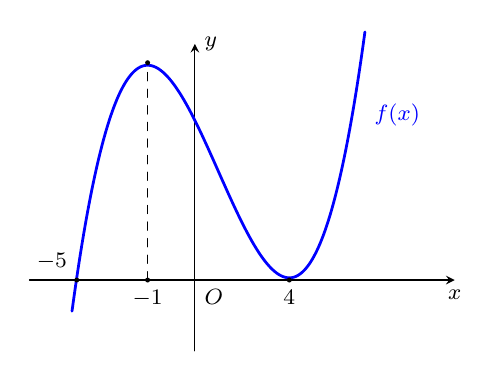
\begin{tikzpicture}[>=stealth,scale=0.6, font=\footnotesize, line join=round,line cap=round]
			% --- Hệ trục tọa độ ---
			\draw[->] (-3.5,0)--(0,0)node[below right]{$O$}--(5.5,0)node[below]{$x$};
			\draw[->] (0,-1.5)--(0,5)node[right]{$y$};
			
			% --- Vẽ đồ thị ---
			\draw[line width=1.0,blue, smooth, samples=150, domain=-2.6:3.6] 
			plot (\x,{1/3*(\x)^3-0.5*(\x)^2-2*(\x)+3.38});
			\node[blue, right] at (3.6,3.5) {$f(x)$};
			
			% --- Các điểm và đường gióng ---
			\draw[dashed] (-1,0)--(-1,4.6);
			
			\fill (-1,4.6) circle (1.5pt);
			\fill (-1,0) circle (1.5pt) node[below] {$-1$};
			\fill (-2.5,0) circle (1.5pt) node[above left] {$-5$};
			\fill (2,0) circle (1.5pt) node[below] {$4$};
	\end{tikzpicture}}
	\loigiai{
		Dựa vào đồ thị hàm số, ta thấy trên khoảng $(-1;4)$, đồ thị đi xuống từ trái sang phải.\\
		Do đó, hàm số $y=f(x)$ nghịch biến trên khoảng $(-1;4)$.
	}
\end{ex}

\begin{ex}%[2H2N2-3]%[TDMZZ22]%[Phạm Hải Dương]
	Trong không gian $Oxyz$, cho hai vectơ $\vec{u}=(1;2;0)$, $\vec{v}=(-2;1;-1)$. Tổng của hai vectơ này có tọa độ là
	\choice
	{$(3;1;1)$}
	{\True $(-1;3;-1)$}
	{$(-3;-1;-1)$}
	{$(1;-2;1)$}
	\loigiai{
		Ta có $\vec{u}+\vec{v}=(1+(-2); 2+1; 0+(-1)) = (-1;3;-1)$.
	}
\end{ex}

\begin{ex}%[2D4N1-4]%[TDMZZ22]%[Phạm Hải Dương]
	Họ nguyên hàm của hàm số $f(x)=\mathrm{e}^x+1$ là
	\choice
	{$F(x)=\mathrm{e}^x+1$}
	{$F(x)=-\mathrm{e}^x+x+C$}
	{$F(x)=\mathrm{e}^x+C$}
	{\True $F(x)=\mathrm{e}^x+x+C$}
	\loigiai{
		Ta có $\displaystyle\int (\mathrm{e}^x+1)\mathrm{\,d}x = \mathrm{e}^x+x+C$.
	}
\end{ex}

\begin{ex}%[2H5N2-2]%[TDMZZ22]%[Phạm Hải Dương]
	Trong không gian $Oxyz$, đường thẳng $d\colon\dfrac{x-1}{3}=\dfrac{y}{4}=\dfrac{z-1}{2}$ có vectơ chỉ phương là
	\choice
	{$\vec{u}_1=(1;0;1)$}
	{$\vec{u}_2=(1;-3;2)$}
	{$\vec{u}_3=(3;2;4)$}
	{\True $\vec{u}_4=(3;4;2)$}
	\loigiai{
		Từ phương trình chính tắc của đường thẳng $d$, ta suy ra một vectơ chỉ phương của đường thẳng là $\vec{u}_4=(3;4;2)$.
	}
\end{ex}

\begin{ex}%[2D4H3-1]%[TDMZZ22]%[Phạm Hải Dương]
	Cho hình phẳng $(H)$ giới hạn bởi các đường $f(x)=x^2+1$, $g(x)=3x-1$. Diện tích hình phẳng $(H)$ bằng
	\choice
	{\True $\dfrac{1}{6}$}
	{$\dfrac{2}{3}$}
	{$\dfrac{1}{3}$}
	{$\dfrac{\pi}{2}$}
	\loigiai{
		Phương trình hoành độ giao điểm của hai đồ thị là
		\[x^2+1=3x-1 \Leftrightarrow x^2-3x+2=0 \Leftrightarrow \hoac{&x=1\\&x=2.}\]
		Diện tích hình phẳng $(H)$ cần tìm là
		\[S = \displaystyle\int\limits_1^2 |(x^2+1)-(3x-1)|\mathrm{\,d}x = \displaystyle\int\limits_1^2 |x^2-3x+2|\mathrm{\,d}x.\]
		Vì $x^2-3x+2 \le 0$ với mọi $x \in [1;2]$ nên:
		\[S = \displaystyle\int\limits_1^2 (-x^2+3x-2)\mathrm{\,d}x = \left.\left(-\dfrac{x^3}{3}+\dfrac{3x^2}{2}-2x\right)\right|_1^2 = \left(-\dfrac{8}{3}+6-4\right) - \left(-\dfrac{1}{3}+\dfrac{3}{2}-2\right) = \dfrac{1}{6}.\]
	}
\end{ex}

\begin{ex}%[2H2H1-2]%[TDMZZ22]%[Phạm Hải Dương]
	\immini[thm]{Cho hình hộp $ABCD. A'B'C'D'$. Khi đó $\overrightarrow{AB} + \overrightarrow{A'D'} + \overrightarrow{DD'}$ bằng vectơ nào dưới đây?
		\choice
		{$\overrightarrow{AB'}$}
		{\True $\overrightarrow{AC'}$}
		{$\vec{0}$}
		{$\overrightarrow{BD}$}}{\begin{tikzpicture}[scale=0.7, font=\footnotesize, line join=round, line cap=round, >=stealth]
			\coordinate (A) at (0,0);
			\coordinate (B) at (-1.5,-1.5);
			\coordinate (C) at (2.5,-1.5);
			\coordinate (D) at ($(A)+(C)-(B)$);
			
			\coordinate (A') at ($(A)+(0,3)$);
			\coordinate (B') at ($(B)+(0,3)$);
			\coordinate (C') at ($(C)+(0,3)$);
			\coordinate (D') at ($(D)+(0,3)$);
			
			\draw (B')--(C')--(D')--(A')--cycle;
			\draw (B')--(B)--(C)--(C') (D')--(D)--(C);
			\draw[dashed] (A')--(A)--(B) (A)--(D);
			
			\fill (A) circle (1.5pt) node[above right] {$A$};
			\fill (B) circle (1.5pt) node[left] {$B$};
			\fill (C) circle (1.5pt) node[below right] {$C$};
			\fill (D) circle (1.5pt) node[right] {$D$};
			\fill (A') circle (1.5pt) node[above left] {$A'$};
			\fill (B') circle (1.5pt) node[left] {$B'$};
			\fill (C') circle (1.5pt) node[below right] {$C'$};
			\fill (D') circle (1.5pt) node[right] {$D'$};
	\end{tikzpicture}}
	\loigiai{
		\begin{center}
			\begin{tikzpicture}[scale=0.7, font=\footnotesize, line join=round, line cap=round, >=stealth]
				\coordinate (A) at (0,0);
				\coordinate (B) at (-1.5,-1.5);
				\coordinate (C) at (2.5,-1.5);
				\coordinate (D) at ($(A)+(C)-(B)$);
				
				\coordinate (A') at ($(A)+(0,3)$);
				\coordinate (B') at ($(B)+(0,3)$);
				\coordinate (C') at ($(C)+(0,3)$);
				\coordinate (D') at ($(D)+(0,3)$);
				
				\draw (B')--(C')--(D')--(A')--cycle;
				\draw (B')--(B)--(C)--(C') (D')--(D)--(C);
				\draw[dashed] (A')--(A)--(B) (A)--(D);
				
				\fill (A) circle (1.5pt) node[above right] {$A$};
				\fill (B) circle (1.5pt) node[left] {$B$};
				\fill (C) circle (1.5pt) node[below right] {$C$};
				\fill (D) circle (1.5pt) node[right] {$D$};
				\fill (A') circle (1.5pt) node[above left] {$A'$};
				\fill (B') circle (1.5pt) node[left] {$B'$};
				\fill (C') circle (1.5pt) node[below right] {$C'$};
				\fill (D') circle (1.5pt) node[right] {$D'$};
			\end{tikzpicture}
		\end{center}
		Trong hình hộp $ABCD. A'B'C'D'$, ta có $\overrightarrow{A'D'} = \overrightarrow{AD}$ và $\overrightarrow{DD'} = \overrightarrow{AA'}$.\\
		Khi đó, áp dụng quy tắc cộng vectơ và quy tắc hình hộp:
		\[\overrightarrow{AB} + \overrightarrow{A'D'} + \overrightarrow{DD'} = \overrightarrow{AB} + \overrightarrow{AD} + \overrightarrow{AA'} = \overrightarrow{AC'}.\]
	}
\end{ex}

\begin{ex}%[2D1H4-1]%[TDMZZ22]%[Phạm Hải Dương]
	Cho hàm số $y=\dfrac{x^2+2x-3}{x^2-5x+4}$ có đồ thị $(C)$. Số đường tiệm cận của đồ thị $(C)$ là
	\choice
	{\True $2$}
	{$3$}
	{$1$}
	{$0$}
	\loigiai{
		Tập xác định $\mathscr{D} = \mathbb{R} \setminus \{1; 4\}$.\\
		Ta phân tích hàm số thành nhân tử: $y = \dfrac{(x-1)(x+3)}{(x-1)(x-4)}$.\\
		Với $x \ne 1$, ta có $y = \dfrac{x+3}{x-4}$.
		\begin{itemize}
			\item Tiệm cận ngang: $\lim\limits_{x \to +\infty} y = \lim\limits_{x \to +\infty} \dfrac{x+3}{x-4} = 1$ và $\lim\limits_{x \to -\infty} y = 1 \Rightarrow y = 1$ là đường tiệm cận ngang của đồ thị hàm số.
			\item Tiệm cận đứng: $\lim\limits_{x \to 4^+} y = \lim\limits_{x \to 4^+} \dfrac{x+3}{x-4} = +\infty \Rightarrow x = 4$ là đường tiệm cận đứng của đồ thị hàm số.\\
			Xét tại $x = 1$: $\lim\limits_{x \to 1} y = \lim\limits_{x \to 1} \dfrac{x+3}{x-4} = \dfrac{4}{-3} = -\dfrac{4}{3} \ne \pm\infty \Rightarrow x = 1$ không phải là tiệm cận đứng.
		\end{itemize}
		Vậy đồ thị hàm số có tổng cộng $2$ đường tiệm cận.
	}
\end{ex}

\begin{ex}%[2D3H1-1]%[TDMZZ22]%[Phạm Hải Dương]
	Cho mẫu số liệu ghép nhóm $M_1$ cùng có $7$ nhóm (các nhóm trong mỗi mẫu số liệu bằng nhau), có phần tử đại diện của hai nhóm thứ $4$ và thứ $5$ lần lượt bằng $8$ và $10$. Đầu mút trái của nhóm thứ $7$ của $M_1$ bằng
	\choice
	{$11$}
	{$15$}
	{\True $13$}
	{$7$}
	\loigiai{
		Gọi độ rộng của mỗi nhóm là $h$.\\
		Vì phần tử đại diện của hai nhóm liên tiếp (nhóm thứ $4$ và thứ $5$) lần lượt là $x_4 = 8$ và $x_5 = 10$, nên ta có
		\[h = x_5 - x_4 = 10 - 8 = 2.\]
		Phần tử đại diện của nhóm thứ $4$ là trung điểm của nhóm thứ $4$ $[a_4; a_5)$, do đó
		\[x_4 = \dfrac{a_4 + a_5}{2} = \dfrac{a_4 + a_4 + h}{2} = a_4 + \dfrac{h}{2} \Rightarrow 8 = a_4 + \dfrac{2}{2} \Rightarrow a_4 = 7.\]
		Các đường mút của các nhóm cách đều nhau một khoảng bằng $h = 2$.\\
		Đầu mút trái của nhóm thứ $7$ chính là $a_7$. Ta có mối liên hệ:
		\[a_7 = a_4 + 3h = 7 + 3 \cdot 2 = 13.\]
		Vậy đầu mút trái của nhóm thứ $7$ bằng $13$.
	}
\end{ex}
\cauds
\begin{ex}%[2D1H5-7]%[Dương Công Tạo]
	Trong mặt phẳng toạ độ $Oxy$, cho hàm số $y = f(x)=x^3 -12x+1$ có đồ thị $(C)$.
	\choiceTF
	{\True $f'(x)=3x^2 -12$}
	{\True Hàm số $f(x)$ nghịch biến trên khoảng $(-2;2)$}
	{\True Hàm số $f(x)$ có hai điểm cực trị}
	{\True $(C)$ có tâm đối xứng là $I(0;1)$}
	\loigiai{
		\begin{itemchoice}
			\itemch Xét hàm số $y = f(x)=x^3 -12x+1$ trên khoảng $(-\infty;+\infty)$.\\
			Ta có $f'(x)=3x^2 -12$.
			\itemch $f'(x)=0\Leftrightarrow 3x^2 -12=0\Leftrightarrow x=\pm 2$.\\
			Bảng biến thiên
			\begin{center}
				
\begin{tikzpicture}[>=stealth]
					\tkzTabInit[nocadre=false,lgt=1.5,espcl=2,deltacl=0.6]{$x$/.7 ,$f'(x)$/.7,$f(x)$/2}
					{$-\infty$ , $-2$ , $2$ , $+\infty$}
					\tkzTabLine{ , + , $0$ , - , $0$ , + , }
					\tkzTabVar{-/$-\infty$ , +/$17$ , -/$-15$ , +/$+\infty$}
				\end{tikzpicture}
			\end{center}
			Dựa vào bảng biến thiên, ta thấy hàm số nghịch biến trên khoảng $(-2;2)$.
			\itemch Dựa vào bảng biến thiên, ta thấy hàm số $f(x)$ có hai điểm cực trị.
			\itemch Ta có $f'(x)=3x^2 -12$; $f''(x)=6x$; $f''(x)=0\Leftrightarrow x=0\Rightarrow y=1$.\\
			Vậy đồ thị $(C)$ có tâm đối xứng là $I(0;1)$.
		\end{itemchoice}
	}
\end{ex}

\begin{ex}%[TDMZZ22]%[Hà Văn Hảo]%[2D4V1-6]
	Một quần thể vi khuẩn ban đầu gồm $200$ vi khuẩn và sau đó bắt đầu tăng trưởng với tốc độ $N'(t) = k e^{-0{,}5t}$ (con/ ngày), với $k$ là hằng số dương, $N(t)$ là số lượng vi khuẩn của quần thể đó sau $t$ ngày. Sau $1$ ngày, số lượng vi khuẩn của quần thể đó đã tăng lên thành $250$ vi khuẩn.
	\choiceTF
	{\True $N(t)$ là một nguyên hàm của $N'(t)$}
	{\True $N(t) = C - 2ke^{-0{,}5t}$ với $C$ là một số thực}
	{\True Tốc độ tăng trưởng của quần thể vi khuẩn giảm dần}
	{\True Trong khoảng thời gian đủ lâu thì số lượng vi khuẩn ổn định và bằng $327$ con (\textit{làm tròn kết quả đến hàng đơn vị})}
	\loigiai{
		\begin{itemchoice}
			\itemch Theo định nghĩa, tốc độ thay đổi của một đại lượng chính là đạo hàm của hàm số biểu thị đại lượng đó theo thời gian.\\
			Do đó $N(t) = \displaystyle\int N'(t)\,\mathrm{d}t $.
			\itemch Ta có $N(t) = \displaystyle\int N'(t)\,\mathrm{d}t = \displaystyle\int k e^{-0{,}5t}\,\mathrm{d}t = k \cdotp \dfrac{e^{-0{,}5t}}{-0{,}5} + C = -2ke^{-0{,}5t} + C$.\\
			Vậy $N(t) = C - 2ke^{-0{,}5t}$.
			\itemch Tốc độ tăng trưởng được cho bởi hàm số $N'(t) = k e^{-0{,}5t}$.\\
			Vì $k > 0$ và đạo hàm của tốc độ tăng trưởng là $N''(t) = -0{,}5k e^{-0{,}5t} < 0$ với mọi $t \ge 0$, nên hàm số $N'(t)$ là hàm nghịch biến.\\
			Do đó, tốc độ tăng trưởng của quần thể vi khuẩn giảm dần theo thời gian.
			\itemch Để xác định số lượng vi khuẩn khi ổn định, ta cần tìm các hằng số $C$ và $k$.\\
			Tại thời điểm $t = 0$ số lượng vi khuẩn là $N(0) = 200$, suy ra
			\allowdisplaybreaks
			\begin{eqnarray*}
				C - 2k e^{0} &=& 200 \\
				\Leftrightarrow C &=& 200 + 2k \quad (1)
			\end{eqnarray*}
			Tại thời điểm $t = 1$ số lượng vi khuẩn là $N(1) = 250$, suy ra
			\allowdisplaybreaks
			\begin{eqnarray*}
				C - 2k e^{-0{,}5} = 250 \quad (2)
			\end{eqnarray*}
			Thay $(1)$ vào $(2)$ ta được
			\[(200 + 2k) - 2ke^{-0,5} = 250 \Leftrightarrow 2k(1 - e^{-0,5}) = 50 \Leftrightarrow 2k = \frac{50}{1 - e^{-0,5}}.\]
			Thay vào $(1)$, ta có $C = 200 + \dfrac{50}{1 - e^{-0{,}5}} \approx 327{,}07$.\\
			Khi thời gian đủ lâu ($t \to +\infty$), số lượng vi khuẩn tiến tới
			\[\lim_{t \to +\infty} N(t) = \lim_{t \to +\infty} \left(C - 2ke^{-0,5t}\right) = C - 0 = C \approx 327{,}07.\]
			Vậy làm tròn đến hàng đơn vị là $327$ con vi khuẩn.
		\end{itemchoice}
	}
\end{ex}

\begin{ex}%[2H5V3-4]%[TDMZZ22]%[Vũ Hồng Toàn]
	Trong không gian $Oxyz$ có đơn vị dài trên mỗi trục là $800$ kilômét, bề mặt Trái Đất được coi là mặt cầu $(S)\colon x^2 + y^2 + z^2 = 64$ và có một vệ tinh địa tĩnh được coi như một hạt có toạ độ $A(0;0;45)$, là một vệ tinh đứng yên so với mặt đất.
	\choiceTF
	{\True Trái Đất được coi là hình cầu có bán kính bằng $6\,400$\,km}
	{\True Điểm $A$ cách bề mặt Trái Đất một khoảng bằng $29\,600$\,km}
	{\True Hình chiếu vuông góc của vệ tinh trên mặt đất là $(0;0;8)$}
	{\True Từ vệ tinh truyền về bề mặt Trái Đất một tín hiệu sóng điện từ với tốc độ $3 \cdot 10^5$\,km/s. Giả sử có hai điểm trên bề mặt Trái Đất nhận được tín hiệu này từ vệ tinh ở hai thời điểm $t_1$ và $t_2$ thì giá trị lớn nhất của $|t_1 - t_2|$ bằng $19$ mili giây (tính theo đơn vị mili giây và làm tròn kết quả đến hàng đơn vị)}
	\loigiai{
		Bề mặt Trái Đất được mô phỏng bởi mặt cầu $(S)\colon x^2 + y^2 + z^2 = 64$ có tâm là gốc tọa độ $O(0;0;0)$ và bán kính $R = 8$ (đơn vị độ dài).
		\begin{itemchoice}
			\itemch Vì đơn vị dài trên mỗi trục là $800$\,km, nên bán kính thực tế của Trái Đất là
			\[8 \cdot 800 = 6\,400\text{ km}.\]
			\itemch Khoảng cách từ vệ tinh $A(0;0;45)$ đến tâm Trái Đất $O(0;0;0)$ là
			\[OA = \sqrt{0^2 + 0^2 + 45^2} = 45 \text{ (đvđd)}.\]
			Khoảng cách từ vệ tinh $A$ đến bề mặt Trái Đất là
			\[OA - R = 45 - 8 = 37 \text{ (đvđd)}.\]
			Khoảng cách thực tế là $37 \cdot 800 = 29\,600$\,(km).
			\itemch Vệ tinh ở vị trí $A(0;0;45)$ nằm trên tia $Oz$. Hình chiếu vuông góc của $A$ trên mặt cầu $(S)$ là giao điểm của đoạn thẳng $OA$ với mặt cầu $(S)$.\\
			Vì $A$ thuộc trục $Oz$ và nằm phía trên mặt đất ($z > 0$), hình chiếu vuông góc của $A$ trên mặt cầu $(S)$ là điểm $H(0;0;8)$.
			\itemch Gọi $M$ là một điểm trên bề mặt Trái Đất nhận được tín hiệu từ vệ tinh $A$.\\
			Để $M$ nhận được tín hiệu trực tiếp từ $A$ thì đoạn thẳng $AM$ không cắt phía trong mặt cầu $(S)$. Do đó, góc $\widehat{AMO} \ge 90^\circ$.\\
			Khoảng cách $AM$ lớn nhất khi $AM$ tiếp xúc với mặt cầu $(S)$, tức là tam giác $AMO$ vuông tại $M$. Khi đó
			\[AM_{\max} = \sqrt{OA^2 - OM^2} = \sqrt{45^2 - 8^2} = \sqrt{1\,961} \text{ (đvđd)}.\]
			Khoảng cách thực tế lớn nhất từ vệ tinh đến điểm nhận tín hiệu là
			\[s_{\max} = \sqrt{1\,961} \cdot 800 \approx 35\,426{,}54\text{ km}.\]
			Khoảng cách thực tế ngắn nhất từ vệ tinh đến điểm nhận tín hiệu (tại điểm cực cận $H$) là $s_{\min} = 29\,600$\,km.\\
			Thời gian truyền tín hiệu lớn nhất và nhỏ nhất lần lượt là
			\[t_{\max} = \dfrac{s_{\max}}{v}, \quad t_{\min} = \dfrac{s_{\min}}{v}.\]
			Giá trị lớn nhất của hiệu thời gian nhận tín hiệu $|t_1 - t_2|$ là
			\[\Delta t_{\max} = t_{\max} - t_{\min} = \dfrac{s_{\max} - s_{\min}}{v} = \dfrac{35\,426{,}54 - 29\,600}{3 \cdot 10^5} \approx 0{,}01942\text{ s} \approx 19\text{ ms}.\]
		\end{itemchoice}
	}
\end{ex}

\begin{ex}%[2D6V1-4]%[TDMZZ22]%[Văn Minh Thoại]
	Cho hai hộp bi riêng biệt, đựng những viên bi cùng kích thước và cùng khối lượng, hộp I đựng $6$ viên bi đỏ và $4$ viên bi xanh, hộp II đựng $7$ viên bi đỏ và $3$ viên bi xanh. Lấy ngẫu nhiên một viên bi từ hộp I bỏ sang hộp II, sau đó lấy ngẫu nhiên một viên bi từ hộp II sang hộp I. Gọi $B$ là biến cố sau khi lấy một viên bi từ hộp I sang hộp II thì hộp II có $7$ đỏ $4$ xanh, $A$ là biến cố sau khi lấy một viên bi từ hộp II bỏ sang hộp I thì hộp I có $6$ viên bi đỏ.
	\choiceTF
	{$\mathrm{P}(A\mid B)=\dfrac{4}{7}$}
	{\True $\mathrm{P}(B\mid A)=\dfrac{1}{4}$}
	{Xác suất để sau cùng hộp I vẫn có $6$ bi đỏ là $\dfrac{6}{11}$}
	{\True $\mathrm{P}(B\mid A)=\dfrac{1}{4}$}
	\loigiai{
		Ta biểu diễn phép thử bằng sơ đồ cây như sau
		\begin{center}
			\begin{tikzpicture}[line join=round, line cap=round, >=stealth, scale=1]
				\node (root) at (0,0) {Trạng thái ban đầu};
				\node (B) at (5,2) {$B$ (Lấy được bi Xanh từ I)};
				\node (Bbar) at (5,-2) {$\overline{B}$ (Lấy được bi Đỏ từ I)};
				
				\node (A1) at (11,3) {$A$ (Lấy lại bi Xanh từ II)};
				\node (Abar1) at (11,1) {$\overline{A}$ (Lấy lại bi Đỏ từ II)};
				
				\node (A2) at (11,-1) {$A$ (Lấy lại bi Đỏ từ II)};
				\node (Abar2) at (11,-3) {$\overline{A}$ (Lấy lại bi Xanh từ II)};
				
				\draw[->] (root) -- (B) node[midway, above left] {$\dfrac{2}{5}$};
				\draw[->] (root) -- (Bbar) node[midway, below left] {$\dfrac{3}{5}$};
				
				\draw[->] (B) -- (A1) node[midway, above left] {$\dfrac{4}{11}$};
				\draw[->] (B) -- (Abar1) node[midway, below left] {$\dfrac{7}{11}$};
				
				\draw[->] (Bbar) -- (A2) node[midway, above left] {$\dfrac{8}{11}$};
				\draw[->] (Bbar) -- (Abar2) node[midway, below left] {$\dfrac{3}{11}$};
			\end{tikzpicture}
		\end{center}
		\begin{itemchoice}
			\itemch Nếu biến cố $B$ đã xảy ra thì hộp II lúc này có tổng cộng $11$ viên bi gồm $7$ đỏ và $4$ xanh.\\
			Để xảy ra biến cố $A$ thì ta phải lấy được viên bi xanh từ hộp II mang về hộp I.\\
			Do đó xác suất có điều kiện $\mathrm{P}(A\mid B)=\dfrac{4}{11}$.
			\itemch Theo tính toán ở trên, nếu biến cố $\overline{B}$ xảy ra thì hộp II sẽ nhận thêm $1$ bi đỏ, lúc này hộp II có $11$ viên bi gồm $8$ đỏ và $3$ xanh.\\
			Để xảy ra biến cố $A$ thì ta phải lấy được viên bi đỏ từ hộp II mang về. Do đó $\mathrm{P}\left(A\mid\overline{B}\right)=\dfrac{8}{11}$.
			\\
			Xác suất để sau cùng hộp I vẫn có $6$ bi đỏ (tức là biến cố $A$ xảy ra) được tính theo công thức xác suất toàn phần
			\[\mathrm{P}(A)=\mathrm{P}(B)\cdot \mathrm{P}(A\mid B)+\mathrm{P}\left(\overline{B}\right)\cdot \mathrm{P}\left(A\mid\overline{B}\right)=\dfrac{2}{5}\cdot\dfrac{4}{11}+\dfrac{3}{5}\cdot\dfrac{8}{11}=\dfrac{8}{55}+\dfrac{24}{55}=\dfrac{32}{55}.\]
			Khi đó
			\[\mathrm{P}(B\mid A)=\dfrac{\mathrm{P}(B)\cdot P(A\mid B)}{\mathrm{P}(A)}=\dfrac{\dfrac{2}{5}\cdot\dfrac{4}{11}}{\dfrac{32}{55}}=\dfrac{\dfrac{8}{55}}{\dfrac{32}{55}}=\dfrac{1}{4}.\]
			\itemch Xác suất để sau cùng hộp I vẫn có $6$ bi đỏ chính là $\mathrm{P}(A)=\dfrac{32}{55}\ne\dfrac{6}{11}$.
			\itemch Theo kết quả tính toán chi tiết ở trên ta đã có $\mathrm{P}(B\mid A)=\dfrac{1}{4}$.
		\end{itemchoice}
	}
\end{ex}
\caukq
\begin{ex}%[2D1H3-6]%[TDMZZ22]%[Lê Hồ Quang Minh]
	Cho hình lăng trụ đều $ABCD. A'B'C'D'$ có diện tích toàn phần bằng $600\text{ cm}^2$. Hãy xác định giá trị lớn nhất của thể tích của $ABCD. A'B'C'D'$ theo đơn vị centimet khối.
	\par\shortans[oly]{1000}
	\loigiai{
		\immini{
			Vì $ABCD. A'B'C'D'$ là hình lăng trụ đều nên đáy $ABCD$ là hình vuông và các cạnh bên vuông góc với đáy.
			Gọi $x$ và $h$ lần lượt là độ dài cạnh đáy hình vuông và chiều cao của khối lăng trụ ($x,h > 0$).\\
			Diện tích toàn phần của hình lăng trụ là
			\[S_{\text{tp}} = 2S_{\text{đáy}} + S_{\text{xq}} = 2x^2 + 4xh.\]
		}{
			\begin{tikzpicture}[scale=0.65, font=\footnotesize, line join=round, line cap=round, >=stealth]
				\coordinate (A) at (0,0);
				\coordinate (B) at (-1.2,-1.5);
				\coordinate (C) at (2.8,-1.5);
				\coordinate (D) at ($(A)+(C)-(B)$);
				\path (A) +(0,4.2) coordinate (A');
				\coordinate (B') at ($(B)+(A')-(A)$);
				\coordinate (C') at ($(C)+(A')-(A)$);
				\coordinate (D') at ($(D)+(A')-(A)$);
				\draw[line width=0.8pt] (A')--(B')--(C')--(D')--cycle;
				\draw[line width=0.8pt] (B)--(C)--(D) (B)--(B') (C)--(C') (D)--(D');
				\draw[dashed, line width=0.7pt] (A)--(B) (A)--(D) (A)--(A');
				\foreach \i/\g in {A/135, B/-135, C/-45, D/45, A'/135, B'/-135, C'/-45, D'/45}
				\fill[black] (\i) circle (1pt) +(\g:2.5mm) node {$\i$};
			\end{tikzpicture}
		}
		\noindent Theo giả thiết, ta có
		\[2x^2 + 4xh = 600 \Rightarrow 4xh = 600 - 2x^2 \Rightarrow h = \dfrac{600 - 2x^2}{4x} = \dfrac{300 - x^2}{2x}.\]
		Vì $h > 0 \Rightarrow 300 - x^2 > 0 \Rightarrow 0 < x < 10\sqrt{3}$.\\
		Thể tích của khối lăng trụ đều là
		\[V = S_{\text{đáy}} \cdot h = x^2 \cdot \dfrac{300 - x^2}{2x} = \dfrac{1}{2}x\cdot\left(300 - x^2\right) = \dfrac{300x - x^3}{2}.\]
		\textbf{Cách 1: Khảo sát hàm số}\\
		Xét hàm số $f(x) = \dfrac{300x - x^3}{2}$ trên khoảng $\left(0; 10\sqrt{3}\right)$, ta
		có \[f'(x) = \dfrac{300 - 3x^2}{2} = 0 \Leftrightarrow 300 - 3x^2 = 0 \Leftrightarrow x^2 = 100 \Rightarrow x = 10.\]
		Bảng biến thiên
		\begin{center}
			
\begin{tikzpicture}
				\tkzTabInit[nocadre=false,lgt=1.5,espcl=2.5,deltacl=0.6]
				{$x$/0.7,$f'(x)$/0.7,$f(x)$/1.5}{$0$,$10$,$10\sqrt{3}$}
				\tkzTabLine{,+,0,-,}   
				\tkzTabVar{-/$0$,+/$1\,000$,-/$0$}
			\end{tikzpicture}
		\end{center}
		Vậy giá trị lớn nhất của thể tích là
		\[V_{\max} = f(10) = \dfrac{300 \cdot 10 - 10^3}{2} = 1\,000\text{ cm}^3.\]
		\textbf{Cách 2: Sử dụng bất đẳng thức Cauchy (AM-GM)}\\
		Ta có
		\allowdisplaybreaks
		\begin{eqnarray*}
			V^2 &=& \dfrac{1}{4}x^2\cdot\left(300 - x^2\right)^2 = \dfrac{1}{8} \cdot \left(2x^2\right) \cdot \left(300 - x^2\right) \cdot \left(300 - x^2\right) \\
			&\le& \dfrac{1}{8} \cdot \left[\dfrac{2x^2 + 300 - x^2 + 300 - x^2}{3}\right]^3= 1\,000\,000 \\
			\Rightarrow V &\le& \sqrt{1\,000\,000} = 1\,000.
		\end{eqnarray*}
		\par Dấu đẳng thức xảy ra khi và chỉ khi $2x^2 = 300 - x^2 \Leftrightarrow 3x^2 = 300 \Leftrightarrow x = 10$ (thỏa mãn).\\
		Vậy giá trị lớn nhất của thể tích khối lăng trụ đều là $1\,000\text{ cm}^3$.
	}
\end{ex}
\begin{ex}%[1H8V6-5]%[TDM31]
	Cho hình lăng trụ $ABC.A'B'C'$ có $\mathrm{d}\big(BB',CC'\big)=6$, số đo các góc nhị diện $\big[A,BB',C\big]$ và $\big[A,CC',B\big]$ lần lượt bằng $120^{\circ}$ và $30^{\circ}$. Hãy tính $\mathrm{d}\big(A,(BCB')\big)$ (\textit{không làm tròn ở các phép tính trung gian và làm tròn kết quả cuối cùng đến hàng phần mười})?
	\par
	\shortans[0]{5,2}
	\loigiai{
		
	}
\end{ex}

\begin{ex}%[0D8C2-7]
	Có $10$ chiếc ghế chia thành hai hàng ngang và thành $5$ cặp đối diện nhau, mỗi chiếc ghế chỉ ngồi được một người. Gọi $T$ là số cách xếp $4$ em lớp A, $3$ em lớp B, $1$ học sinh lớp C, $1$ học sinh lớp D, $1$ học sinh lớp E vào $10$ ghế này sao cho không có học sinh nào cùng lớp ngồi đối diện nhau. Hãy tính $\dfrac{T}{1000}$ (\textit{làm tròn kết quả đến hàng đơn vị}).
	\begin{center}
		\begin{tikzpicture}[line join = round, line cap = round,>=stealth,font=\footnotesize,scale=0.8]
			\foreach \x in {0,2,4,6,8} \draw (\x,0) rectangle (\x+1,1);
			\foreach \x in {0,2,4,6,8} \draw (\x,-0.5) rectangle (\x+1,-1.5);  
		\end{tikzpicture}
	\end{center}
	\par\shortans{2972}
	\loigiai{
		Ta coi $4$ em học sinh lớp A như nhau, $3$ 3m học sinh lớp B như nhau. Coi $2$ ghế đối diện là một cột, như vậy ta có $5$ cột.
		\begin{itemize}
			\item Đầu tiên ta chọn $4$ cột xếp $4$ em lớp A, mỗi cột xếp một em, có $\mathrm{C}^4_5\cdot 2^4$ cách xếp.
			\item Tiếp theo ta xếp $3$ học sinh lớp B. Có các cách xếp sau
			\begin{itemize}
				\item $3$ học sinh lớp B xếp vào $4$ ô đối diện đã xếp học sinh lớp A. Có $\mathrm{C}^3_4$ cách.
				\item $2$ học sinh lớp B xếp vào $4$ ô đối diện đã xếp học sinh lớp A, $1$ học sinh lớp B còn lại xếp vào $2$ cột tự do. Có $\mathrm{C}^2_4\cdot \left(\mathrm{C}^1_2\cdot 2^1\right)$ cách.
				\item $1$ học sinh lớp B xếp vào $4$ ô đối diện đã xếp học sinh lớp A, $2$ học sinh lớp B còn lại xếp vào $2$ cột tự do. Có $\mathrm{C}^1_4\cdot \left(\mathrm{C}^2_2\cdot 2^2\right)$ cách.
			\end{itemize}
			\item Tiếp theo ta xếp $1$ học sinh lớp C, $1$ học sinh lớp D, $1$ học sinh lớp E vào $3$ ghế trống. Có $3!$ cách.
		\end{itemize}
		Vậy, số cách xếp thỏa mãn là
		$$T=\left[\mathrm{C}^4_5\cdot 2^4\cdot \left(\mathrm{C}^3_4+\mathrm{C}^2_4\cdot \left(\mathrm{C}^1_2\cdot 2^1\right)+\mathrm{C}^1_4\cdot \left(\mathrm{C}^2_2\cdot 2^2\right) \right)\cdot 3!\right] \cdot 4!\cdot 3!=2\,972\,160.$$
		Do đó $\dfrac{T}{1000} =2\,972{,}16\approx 2\,972$.
	}
\end{ex}

\begin{ex}%[2D6C2-4]%[TDMZZ22]%[Nguyễn Đức Tuấn Anh]
	Theo thống kê hiện tại có một dịch bệnh X rất nguy hiểm và đang có $3\%$ dân số thật sự mắc bệnh này. Một công ty có đề xuất một loại dụng cụ TEST X cho khả năng phát hiện chuẩn đến $92\%$ một loại bệnh X (tức là một người bị bệnh X khi dùng dụng cụ TEST X sẽ cho xác suất dương tính là $92\%$). Tuy nhiên, TEST X cũng cho kết quả \lq\lq dương tính giả\rq\rq\ cho một người không bị bệnh X tới $4\%$ (tức là một người không bị bệnh X mà dùng TEST X sẽ cho kết quả dương tính là $4\%$). Một người dùng TEST X này $5$ lần liên tiếp, kết quả các lần TEST là độc lập với nhau. Gọi $p$ là xác suất để người này nhận được kết quả dương tính đúng $2$ lần. Hãy tính $10\,000p$ (\textit{làm tròn kết quả đến hàng đơn vị})?
	\par\shortans[]{139}
	\loigiai{
		Gọi $B$ là biến cố \lq\lq Người được chọn thực sự mắc bệnh X\rq\rq. Ta có $\mathrm{P}(B) = 0{,}03$ và $\mathrm{P}(\overline{B}) = 0{,}97$.\\
		Gọi $A$ là biến cố \lq\lq Người này nhận được kết quả dương tính đúng $2$ lần trong $5$ lần test\rq\rq.\\
		Nếu người đó mắc bệnh X, xác suất mỗi lần test dương tính là $0{,}92$.\\
		Vì các lần test độc lập, xác suất để người này test dương tính đúng $2$ lần là
		\[ \mathrm{P}\left(A \mid B\right) = \mathrm{C}_5^2 \cdot (0{,}92)^2 \cdot (1 - 0{,}92)^3 = 10 \cdot 0{,}92^2 \cdot 0{,}08^3. \]
		Nếu người đó không mắc bệnh X, xác suất mỗi lần test dương tính là $0{,}04$. \\
		Tương tự, xác suất để người này test dương tính đúng $2$ lần là
		\[ \mathrm{P}\left(A \mid \overline{B}\right) = \mathrm{C}_5^2 \cdot (0{,}04)^2 \cdot (1 - 0{,}04)^3 = 10 \cdot 0{,}04^2 \cdot 0{,}96^3. \]
		Theo công thức xác suất toàn phần, xác suất $p$ để người này nhận kết quả dương tính đúng $2$ lần là
		\allowdisplaybreaks
		\begin{align*}
			p = \mathrm{P}(A) &= \mathrm{P}(B) \cdot \mathrm{P}(A \mid B) + \mathrm{P}\left(\overline{B}\right) \cdot \mathrm{P}\left(A \mid \overline{B}\right) \\
			&= 0{,}03 \cdot 10 \cdot 0{,}92^2 \cdot 0{,}08^3 + 0{,}97 \cdot 10 \cdot 0{,}04^2 \cdot 0{,}96^3 \\
			&\approx 0{,}01386.
		\end{align*}
		Vậy $10\,000p \approx 139$.
	}
\end{ex}
\begin{ex}
	content
\end{ex}
\begin{ex}%[2H5C3-4]%[TDM42]%[Nguyễn Văn Sang]
	Trong không gian $Oxyz$ có đơn vị dài trên mỗi trục là centimet, cho một vật chuyển động tự do trên một mặt cầu cố định sao cho nó có các thành phần tọa độ luôn dương. Biết vật cách bốn mặt phẳng $(\alpha): x=10, (\beta): x=130, (\gamma): z=0, (\delta): y=10$ những khoảng xa nhất lần lượt là $100\text{ cm}, 60\text{ cm}, 80\text{ cm}, 70\text{ cm}$. Hãy tính theo đơn vị centimet khoảng cách lớn nhất giữa vật và gốc $O$ \textit{(không làm tròn ở các phép tính trung gian và làm tròn kết quả cuối cùng đến hàng đơn vị)}?
	\par\shortans[0]{144}
	\loigiai{
		\textbf{Bước 1: Tư duy phân tích hình học về khoảng cách xa nhất đến một mặt phẳng}\\
		Gọi mặt cầu cố định mà vật chuyển động trên đó là $(S)$ có tâm $I(x_0; y_0; z_0)$ và bán kính $R$.
		Vì một điểm $M$ bất kỳ di động trên mặt cầu $(S)$, khoảng cách từ $M$ đến một mặt phẳng $(P)$ bất kỳ luôn tuân theo quy luật hình học trực quan: điểm nằm xa mặt phẳng nhất chính là điểm nằm trên đường thẳng đi qua tâm $I$ và vuông góc với $(P)$.\\
		Do đó, khoảng cách lớn nhất từ vật đến mặt phẳng $(P)$ được tính bằng công thức:
		$$d_{\max}(M, (P)) = d(I, (P)) + R$$
		\textbf{Bước 2: Lập hệ phương trình xác định tâm và bán kính mặt cầu}\\
		Theo đề bài, đề cho khoảng cách lớn nhất từ vật đến bốn mặt phẳng $(\alpha), (\beta), (\gamma), (\delta)$. Áp dụng công thức trên kèm điều kiện các thành phần tọa độ của vật luôn dương ($x_0, y_0, z_0 > R$), ta có hệ thức sau:
		\begin{itemize}
			\item Với mặt phẳng $(\alpha): x = 10 \implies |x_0 - 10| + R = 100 \quad (1)$
			\item Với mặt phẳng $(\beta): x = 130 \implies |x_0 - 130| + R = 60 \quad (2)$
			\item Với mặt phẳng $(\gamma): z = 0 \implies z_0 + R = 80 \quad (3)$
			\item Với mặt phẳng $(\delta): y = 10 \implies |y_0 - 10| + R = 70 \quad (4)$
		\end{itemize}
		Từ hai phương trình $(1)$ và $(2)$, ta trừ vế theo vế để triệt tiêu bán kính $R$
		$$|x_0 - 10| - |x_0 - 130| = 100 - 60 = 40 \quad (*)$$
		Giải phương trình $(*)$ với điều kiện thành phần tọa độ dương ($10 < x_0 < 130$)
		$$(x_0 - 10) - (130 - x_0) = 40 \iff 2x_0 - 140 = 40 \iff 2x_0 = 180 \iff x_0 = 90$$
		Thay $x_0 = 90$ ngược lại vào phương trình $(1)$, ta tìm được bán kính $R$
		$$|90 - 10| + R = 100 \iff 80 + R = 100 \iff R = 20 \text{ cm}.$$
		Có được $R = 20$, ta lần lượt thay vào phương trình $(3)$ và $(4)$ để tìm $y_0$ và $z_0$
		\begin{itemize}
			\item Từ $(3) \implies z_0 + 20 = 80 \iff z_0 = 60$
			\item Từ $(4) \implies |y_0 - 10| + 20 = 70 \iff |y_0 - 10| = 50 \iff y_0 = 60$ (loại nghiệm $y_0 = -40$ vì tọa độ phải dương).
		\end{itemize}
		Như vậy, mặt cầu cố định $(S)$ có tâm $I(90; 60; 60)$ và bán kính $R = 20$ cm.\\
		\textbf{Bước 3: Tư duy trực quan tìm khoảng cách lớn nhất đến gốc tọa độ $O$}\\
		Xét một điểm $M$ di động trên mặt cầu $(S)$ tâm $I$, khoảng cách từ $M$ đến gốc tọa độ cố định $O$ nằm ngoài mặt cầu đạt giá trị lớn nhất khi và chỉ khi ba điểm $O, I, M$ thẳng hàng theo thứ tự $O \to I \to M$ (tức là $M$ nằm ở mặt đối diện xa nhất của mặt cầu so với gốc $O$).
		\begin{center}
			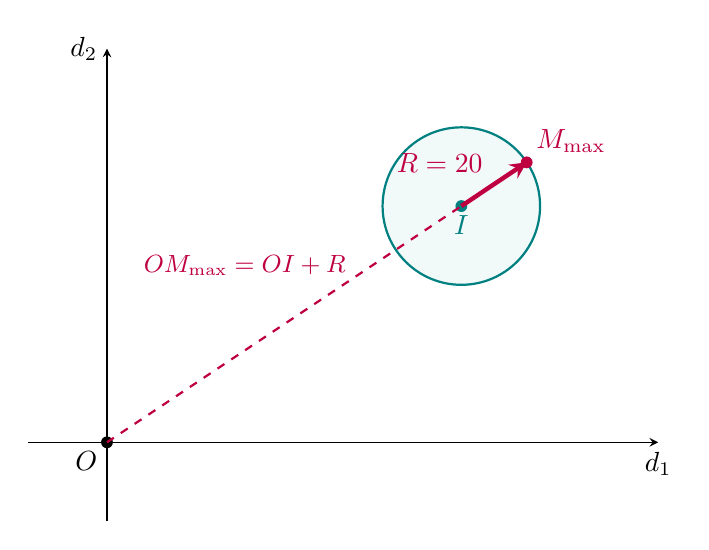
\begin{tikzpicture}[scale=0.05, >=stealth]
				% Mặt phẳng phẳng cắt qua tia OI
				\fill[teal!5] (90,60) circle (20);
				\draw[thick, teal] (90,60) circle (20);
				
				\coordinate (O) at (0,0);
				\coordinate (I) at (90,60);
				% Điểm M_max nằm trên đường thẳng kéo dài OI
				% OI dài 108.16, cộng thêm R=20
				coordinate (Mmax) at (106.6, 71.1);
				
				\draw[black, ->] (-20,0) -- (140,0) node[below] {$d_1$};
				\draw[black, ->] (0,-20) -- (0,100) node[left] {$d_2$};
				
				\fill[black] (O) circle (1.5) node[below left] {$O$};
				\fill[teal] (I) circle (1.5) node[below] {$I$};
				
				\draw[purple, dashed, thick] (O) -- (I);
				\draw[purple, ultra thick, ->] (I) -- (106.6, 71.1) node[midway, above left] {$R=20$};
				\fill[purple] (106.6, 71.1) circle (1.5) node[above right] {$M_{\max}$};
				
				\node[purple, font=\small, align=left] at (35,45) {$OM_{\max} = OI + R$};
			\end{tikzpicture}
		\end{center}
		Khi đó, khoảng cách cực đại được tính bằng tổng độ dài đoạn nối tâm và bán kính:
		$$OM_{\max} = OI + R$$
		Tính độ dài đoạn thẳng $OI$
		$$OI = \sqrt{90^2 + 60^2 + 60^2} = \sqrt{8100 + 3600 + 3600} = \sqrt{15300} = 30\sqrt{17} \text{ cm}$$
		\textbf{Bước 4: Tính toán kết quả cuối cùng}
		Khoảng cách lớn nhất cần tìm là
		$$OM_{\max} = 30\sqrt{17} + 20 \approx 123,6932 + 20 \approx 144 \text{ cm}.$$
	}
\end{ex}